% fig5_ffi_boundary.tex — Figure 4 (column width)
% New 2026-09-15 (COMSI-2026-04-0112, design/ieee-figure-redesign):
% illustrates Sec. 4.7 "Polyglot Deployment: The FFI Trust Boundary",
% previously unillustrated. Shows the trust boundary, not a proof case:
% the Rust gateway protects Verdict construction; routing enforcement
% downstream is an infrastructure obligation, stated in the bottom line.
\documentclass[border=2pt]{standalone}
\usepackage{tikz}
\usetikzlibrary{arrows.meta,positioning,fit,calc}
\begin{document}
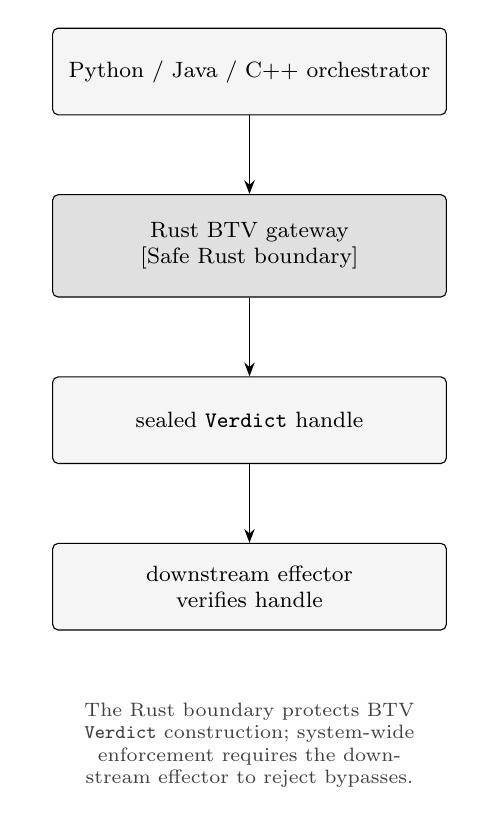
\begin{tikzpicture}[
  font=\footnotesize,
  box/.style={draw, rounded corners=2pt, align=center, inner sep=5pt,
    minimum width=50mm, minimum height=11mm, fill=black!04},
  gw/.style={draw, rounded corners=2pt, align=center, inner sep=5pt,
    minimum width=50mm, minimum height=13mm, fill=black!12},
  arr/.style={-{Stealth[length=5pt]}, semithick},
  note/.style={align=center, font=\scriptsize, text=black!75}
]

\node[box] (orch) at (0,0) {Python / Java / C++ orchestrator};
\node[gw, below=10mm of orch] (gw) {Rust BTV gateway\\ \footnotesize[Safe Rust boundary]};
\node[box, below=10mm of gw] (sealed) {sealed \texttt{Verdict} handle};
\node[box, below=10mm of sealed] (eff) {downstream effector\\ verifies handle};

\draw[arr] (orch) -- (gw);
\draw[arr] (gw) -- (sealed);
\draw[arr] (sealed) -- (eff);

\node[note, below=8mm of eff, text width=54mm]
  {The Rust boundary protects BTV \texttt{Verdict} construction; system-wide enforcement requires the downstream effector to reject bypasses.};

\end{tikzpicture}
\end{document}
